Schaltwerke (sequentielle Logik) können im Gegensatz zu 
Schaltnetzen (kombinatorische Logik) deren Zustände
speichern. Als Grundlage dienen hierfür Flip-Flops,
also bistabile Kippstufen, die es in diversen
Ausführungen gibt - beispielsweise existieren unterschiedliche
Steuerungsarten (zustands- oder flankengesteuert). 
Elementar ist hierbei das RS-Flip-Flop wie es in
\autoref{fig:rs_flip} zu sehen ist. Hierbei wurde jenes
mittels NOR-Gattern realisiert; anstelle hätten auch
NAND-Gatter verwendet werden können.
\begin{figure}[H]
  \centering
    % 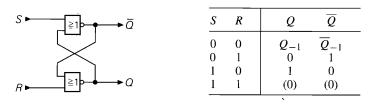
\includegraphics[width=0.95\textwidth]{./figures/rs_ff.png}
    \caption{Diese Schaltung zeigt den Aufbau eines
    RS-Flip-Flops aus NOR-Gattern mit Eingängen $R$ und
    $S$ sowie Ausgängen $Q$ und $\Bar{Q}$ \cite{tietze}
  }
  \label{fig:rs_flip}
\end{figure}
Dabei handelt es sich um ein zustandsgesteuertes
Flip-Flop mit den Eingängen $R$ und $S$ sowie
Ausgängen $Q$ und $\Bar{Q}$, wobei dieses
transparent ist, da Änderungen vom Ein- auf den
Ausgang sofort übertragen werden.
Ein Flip-Flop kann nun mit einem zusätzlichen
Eingang, dem Takt, auch Clock (C),
angesteuert werden. Wenn nun zusätzlich zwei Flips-Flops miteinander
seriell verbunden werden und der Takt am Eingang des zweiten Flip-Flops 
negiert wird, kann man ein Master-Slave Flip-Flop erhalten, welches
zweiflankengesteuert und nicht-transparent ist; d.h. dass am Master, dem erste Flip-Flop, die
Signale der Eingänge bei steigender Flanke eingelesen/zwischengespeichert
und an den Slave, den hinteren Flip-Flop, bei fallender Flanke
übertragen werden, wobei der Eingang dabei verriegelt ist.
Somit sind Eingang und Ausgang also getrennt.
Wenn weiters die Ausgänge auf die Eingänge rückgekoppelt
werden, erhält man ein zweiflankengesteuertes JK-Master-Slave
Flip-Flop mit Eingängen $J$ und $K$, wie es in \autoref{sec:Vorbereitung} 
(Vorbereitung) inklusive
der zugehörigen Wahrheitstabelle dargestellt wird. Aufgrund
der Rückkopplung tritt bei $J=K=1$  Togglen auf (an der negativen Flanke des Takts),
was das Kippen des vorherigen Zustands beschreibt. Diese Konstellation der
Eingangszustände war ohne Rückkopplung nicht definiert beziehungsweise verboten.

Anwendungen finden Flip-Flops unter anderem für Zähler (wie in dieser
Laborübung) oder für Schieberegister. Dabei stellen die Flip-Flops
Speicherelemente für die Zustände dar, welche mittels der
anliegenden Taktung
verändert werden können. 
